\ExamPart{Câu trắc nghiệm nhiều phương án lựa chọn}{3}{Mỗi câu hỏi thí sinh chỉ chọn một phương án.}

\NQuestion Cho hàm số $y=x^2-6x+5$. Tọa độ đỉnh của parabol là

\ChoicesOneLine{$(3;-4)$.}{$(-3;4)$.}{$(3;4)$.}{$(-3;-4)$.}

\NQuestion Cho phương trình $x^2-5x+m=0$. Với giá trị nào của $m$ thì phương trình có hai nghiệm phân biệt?

\ChoicesOneLine{$m<\dfrac{25}{4}$.}{$m\le \dfrac{25}{4}$.}{$m>\dfrac{25}{4}$.}{$m=\dfrac{25}{4}$.}

\NQuestion Trong mặt phẳng tọa độ $Oxy$, cho hai điểm $A(1;2)$ và $B(5;-1)$. Độ dài đoạn thẳng $AB$ bằng

\ChoicesOneLine{$5$.}{$4$.}{$\sqrt{13}$.}{$\sqrt{34}$.}

\NQuestion Trong mặt phẳng tọa độ $Oxy$, đường thẳng đi qua hai điểm $M(0;1)$ và $N(2;5)$ có hệ số góc bằng

\ChoicesOneLine{$2$.}{$\dfrac{1}{2}$.}{$-2$.}{$4$.}

\NQuestion Cho đường tròn có tâm $I(-2;3)$ và bán kính $R=4$. Phương trình đường tròn là

\ChoicesTwoLines
{$(x+2)^2+(y-3)^2=4$.}
{$(x-2)^2+(y+3)^2=16$.}
{$(x+2)^2+(y-3)^2=16$.}
{$(x-2)^2+(y+3)^2=4$.}

\NQuestion Cho elip $(E):\dfrac{x^2}{49}+\dfrac{y^2}{9}=1$. Tọa độ các tiêu điểm của elip là

\ChoicesTwoLines
{$F_1(-4;0),\,F_2(4;0)$.}
{$F_1(-5;0),\,F_2(5;0)$.}
{$F_1(-2\sqrt{10};0),\,F_2(2\sqrt{10};0)$.}
{$F_1(0;-2\sqrt{10}),\,F_2(0;2\sqrt{10})$.}

\NQuestion Cho hàm số bậc hai $y=f\left(x\right)$ có đồ thị như hình bên. Số nghiệm của phương trình $f\left(x\right)=0$ là

\begin{center}
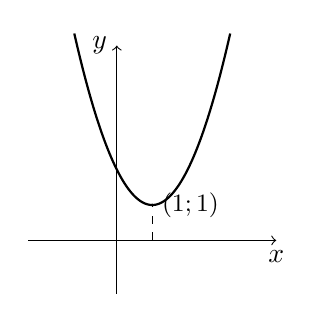
\begin{tikzpicture}[scale=0.45]
    \draw[->] (-2.5,0) -- (4.5,0) node[below] {$x$};
    \draw[->] (0,-1.5) -- (0,5.5) node[left] {$y$};

    \draw[thick, domain=-1.2:3.2, samples=200] plot (\x,{(\x-1)^2+1});
    \draw[dashed] (1,0) -- (1,1);
    \fill (1,1) circle (1.2pt);
    \node[right] at (1,1) {\small $(1;1)$};
\end{tikzpicture}

\end{center}

\ChoicesOneLine{0.}{1.}{2.}{3.}

\NQuestion Trong các số tự nhiên có hai chữ số khác nhau lập từ các chữ số $0,1,2,3,4$, có bao nhiêu số chia hết cho $2$?

\ChoicesOneLine{8.}{10.}{12.}{14.}

\NQuestion Trong mặt phẳng tọa độ $Oxy$, cho đường thẳng $d: x-2y+3=0$. Phương trình đường thẳng song song với $d$ và đi qua điểm $A(1;1)$ là

\ChoicesOneLine{$x-2y+1=0$.}{$x-2y+3=0$.}{$2x-y-1=0$.}{$x+2y-3=0$.}

\NQuestion Diện tích hình chữ nhật có chiều dài $8$ và chiều rộng $5$ là

\ChoicesOneLine{13.}{26.}{40.}{80.}
